\section{New Layout Engine}
\label{prototype:NewLayoutEngine}
Currently my graph layout engine uses a single iteration of the F-Cose layout algorithm (designed by  i-Vis Lab in Bilkent). This layout (in simple terms) randomly spaces each node and then converges them to try to match the connecting edge length to a specified integer which makes the graph more visually appealing. 

While this layout has many advantages such as:
\begin{itemize}
	\item Ability to specify the location of certain 'static' nodes and generate locations for other nodes around them
	\item Keeping edge lengths even between nodes
	\item Visually appealing layouts
	\item Runs very quickly and is performant
\end{itemize}

It also has a number of downsides:

\begin{itemize}
	\item Algorithm has no concept of overlapping edges which are both visually obtrusive and make it harder to follow paths between nodes
	\item Algorithm is static - once it is run there is no further interactivity and nodes have to each be manually moved if changes are wanted
\end{itemize}

To help mitigate these downsides I have designed a 2 stage approach to laying out nodes:

	1) This first stage is effectively the same as my prior layout engine. A Fcose layout is run on the nodes, static nodes are sent to their saved position and all others move around them (unless otherwise specified). 
	2) Once the 'stage Is set' (and is looking like the top image) I then run a different layout - Cola, which continues to run for the lifetime of the page being open

Cola is a force directed physics simulation written by Tim Dwyer. Unlike Fcose which purely applies mathematical transformations to nodes at 'random', Cola simulates tension and gravity impacting the nodes. Like with many natural images, humans are very aesthetically drawn to designs produced by natural forces (also seen by the golden ratio). Whilst cola struggles with the initial placement of nodes in a sensible way (hence the need for my first step) it can then continually run on the nodes, simulating their interactions with the users mouse. As nodes are dragged around, they pull their connected children and push around their neighbours as they collide which doesn’t just provide a satisfying organisation method but Is also therapeutic to use just dragging notes around

The graph view of the application Obsidian was a large inspiration for this 'live' design, also infinitely running it provides similar benefits however I think my implementation is better in some ways especially the satisfying way nodes naturally move 


An example of the prior layout engine which has overlapping nodes, nodes trying to combine and nodes sent far from the centre due to tension constraints:
\begin{figure}[H]
    \centering
    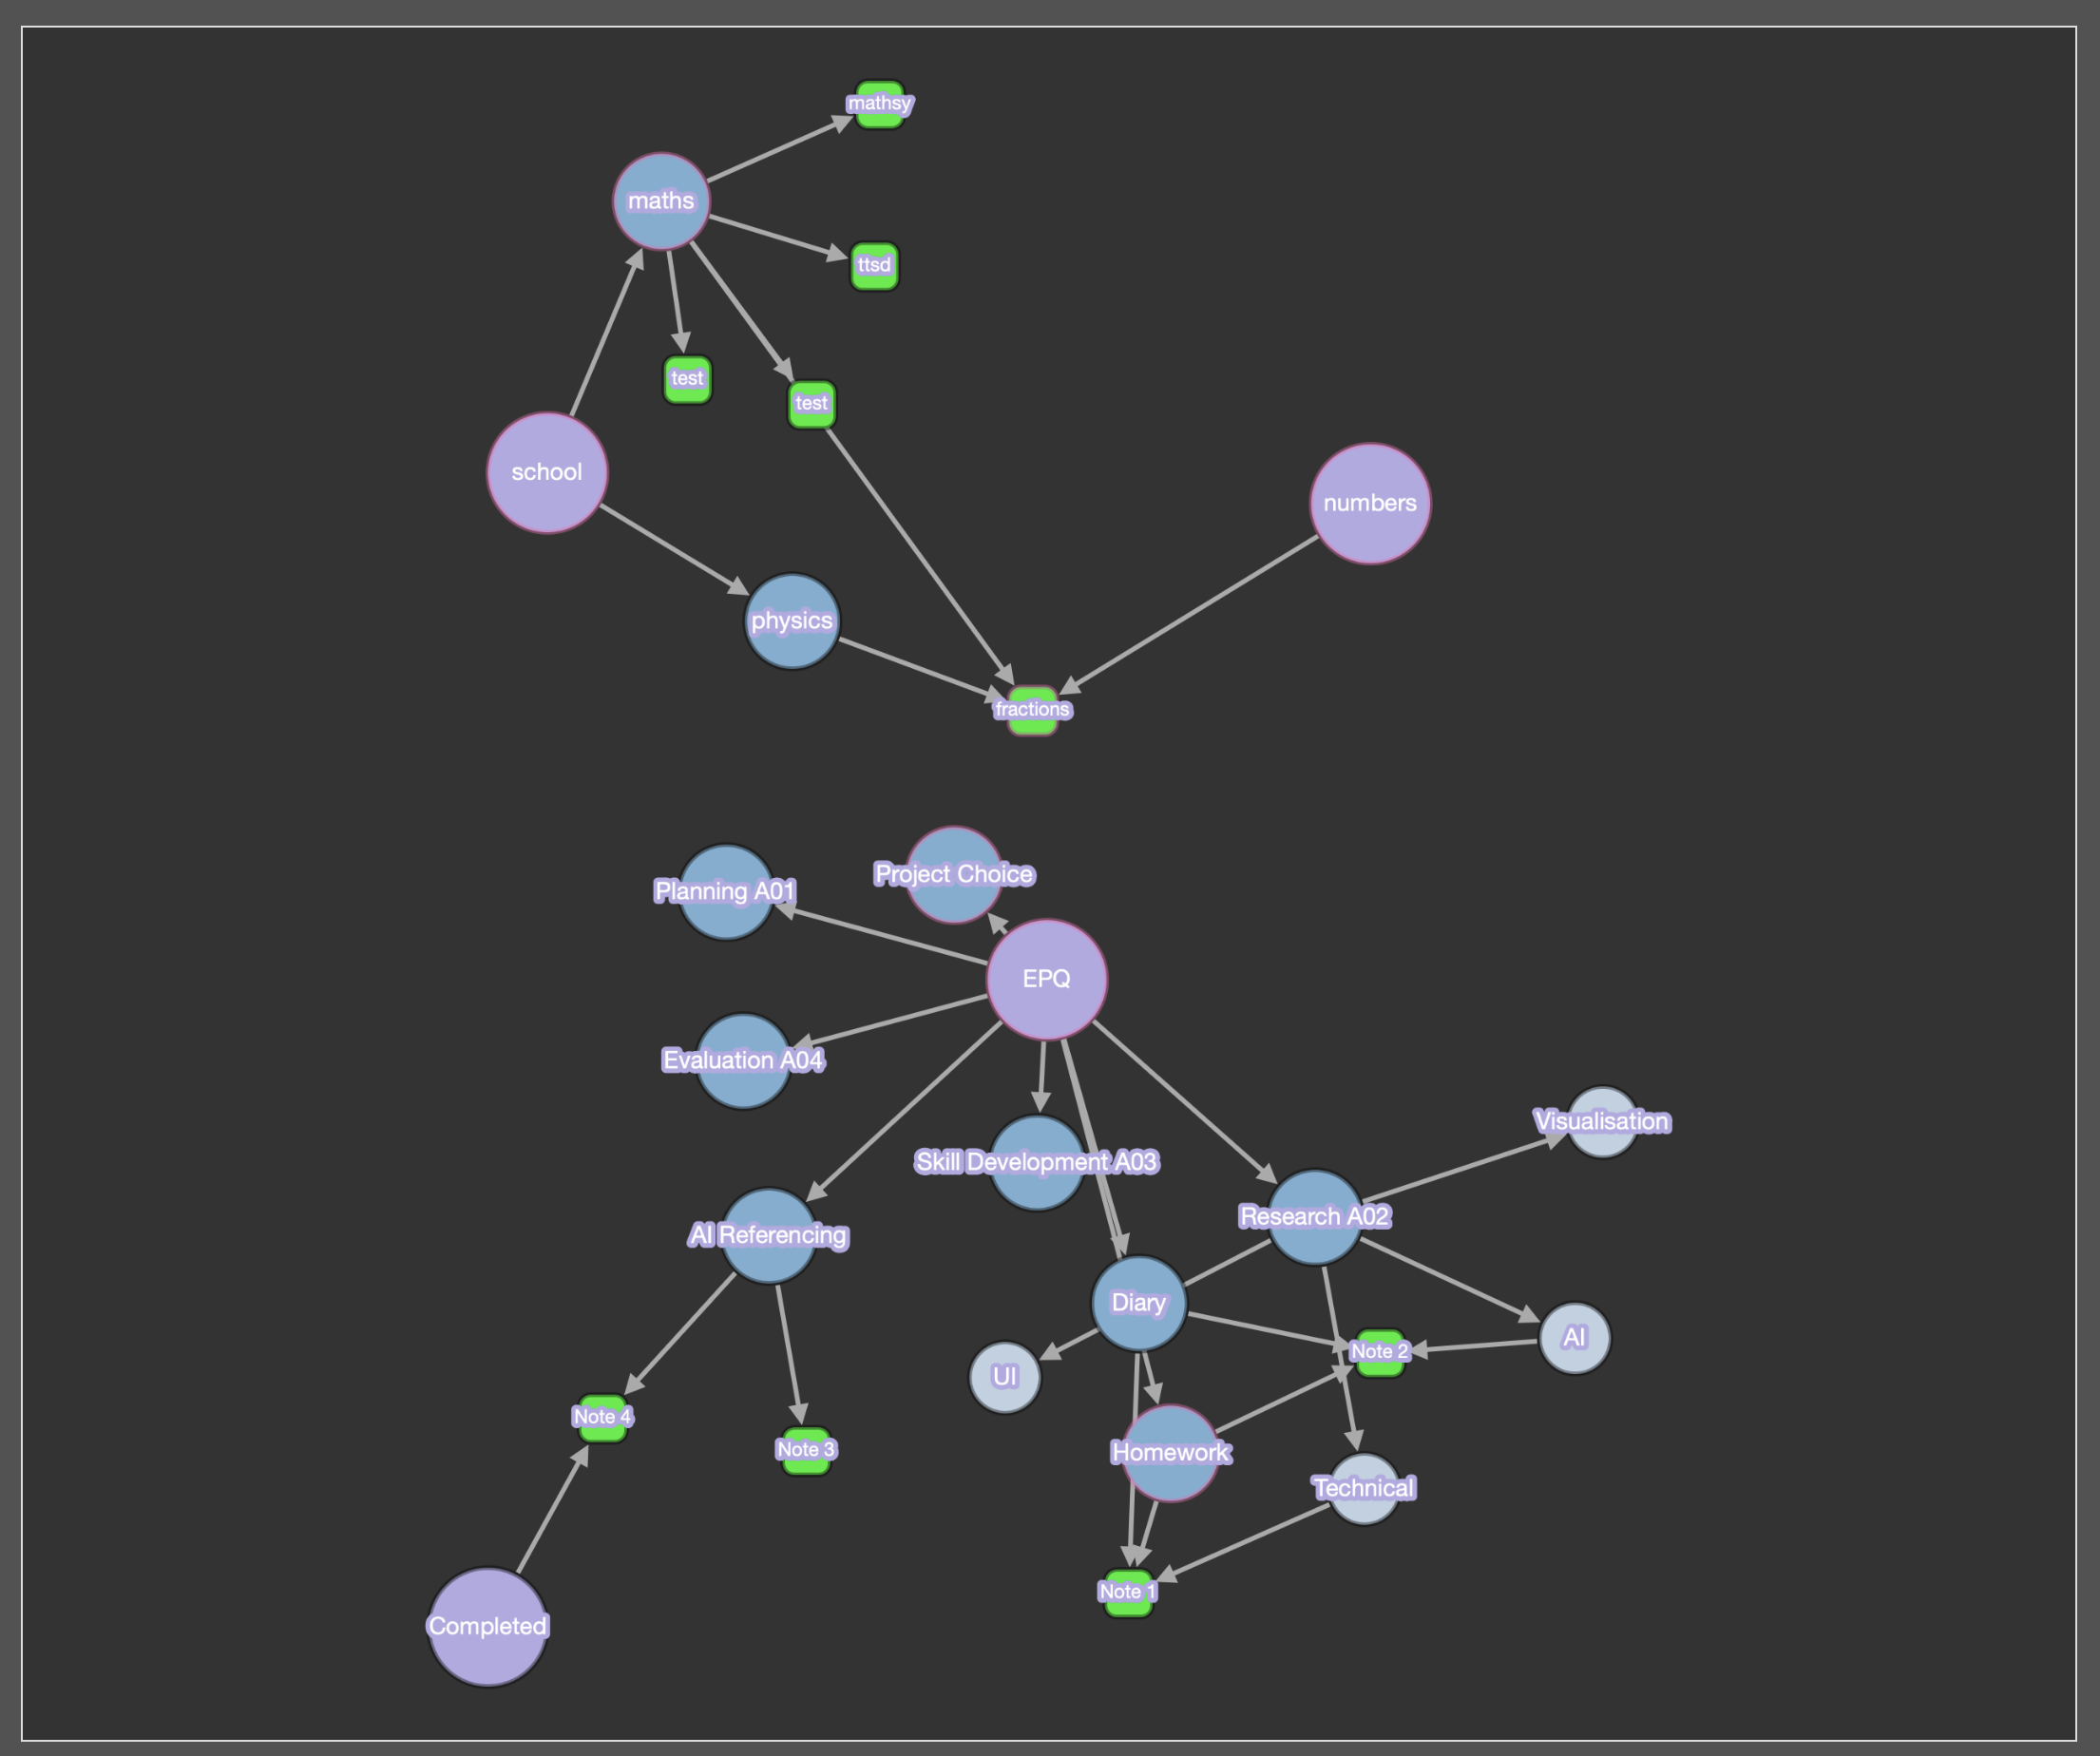
\includegraphics[width=0.8\textwidth]{Prototype/13_NewLayoutEngine/media/before.png}
    \caption{Prior layout algorithm}
\end{figure}

The same nodes on my new layout system - I'm sure you can agree it's cleaner and clearer:
\begin{figure}[H]
    \centering
    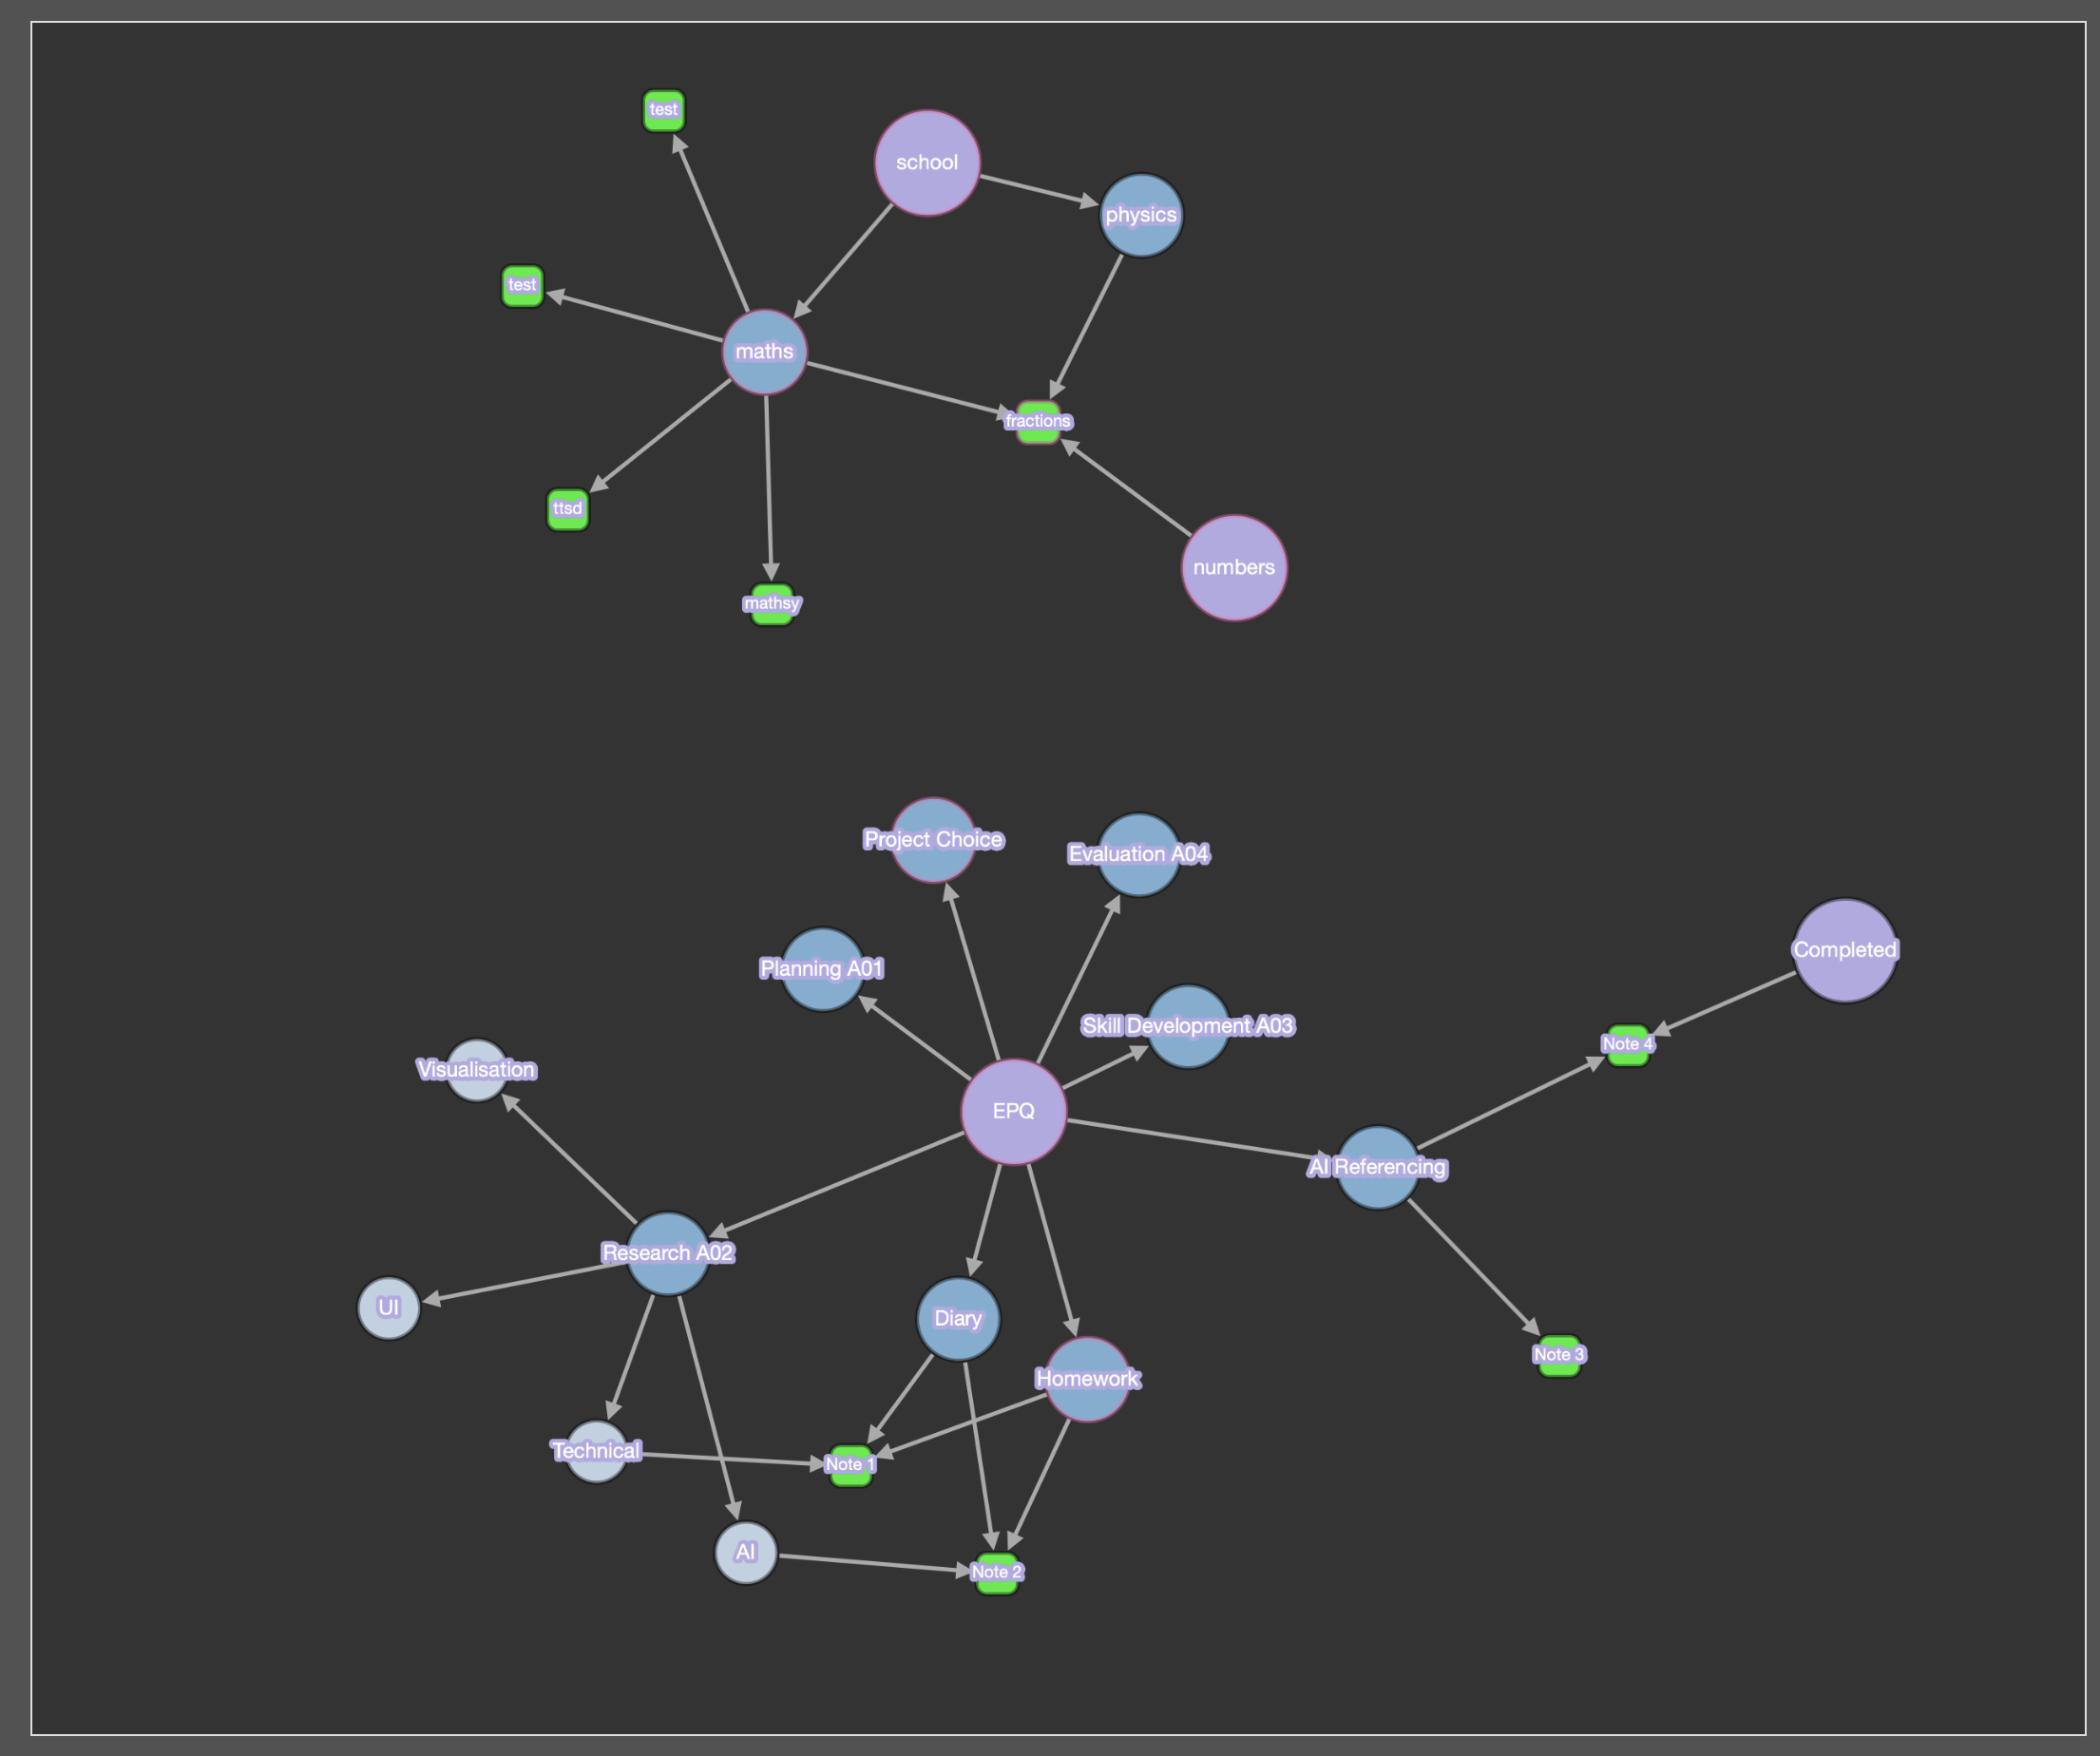
\includegraphics[width=0.8\textwidth]{Prototype/13_NewLayoutEngine/media/after.png}
    \caption{New layout algorithm}
\end{figure}
